\section{Neuronale Netze} %TODO: Absplitten

\subsection{Aufbau und Namenskonvetionen}
\begin{figure}[ht!]
\label{fig:MLP}
  \centering
    \def\layersep{2.5cm}

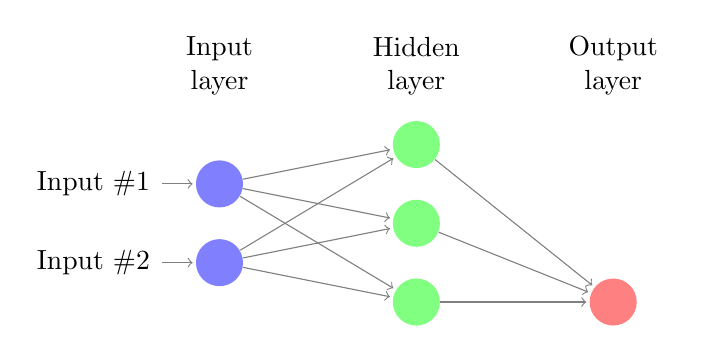
\begin{tikzpicture}[shorten >=1pt,->,draw=black!50, node distance=\layersep]
    \tikzstyle{every pin edge}=[<-,shorten <=1pt]
    \tikzstyle{neuron}=[circle,fill=black!25,minimum size=17pt,inner sep=0pt]
    \tikzstyle{input neuron}=[neuron, fill=blue!50];
    \tikzstyle{output neuron}=[neuron, fill=red!50];
    \tikzstyle{hidden neuron}=[neuron, fill=green!50];
    \tikzstyle{annot} = [text width=4em, text centered]

    % Draw the input layer nodes
    \foreach \name / \y in {1,...,2}
    % This is the same as writing \foreach \name / \y in {1/1,2/2,3/3,4/4}
        \node[input neuron, pin=left:Input \#\y] (I-\name) at (0,-\y) {};

    % Draw the hidden layer nodes
    \foreach \name / \y in {1,...,3}
        \path[yshift=0.5cm]
            node[hidden neuron] (H-\name) at (\layersep,-\y cm) {};

    % Draw the output layer node
    %\node[output neuron,pin={[pin edge={->}]right:Output}, right of=H-3] (O) {};
    \node[output neuron, right of=H-3] (O) {};

    % Connect every node in the input layer with every node in the
    % hidden layer.
    \foreach \source in {1,...,2}
        \foreach \dest in {1,...,3}
            \path (I-\source) edge (H-\dest);

    % Connect every node in the hidden layer with the output layer
    \foreach \source in {1,...,3}
        \path (H-\source) edge (O);

    % Annotate the layers
    \node[annot,above of=H-1, node distance=1cm] (hl) {Hidden layer};
    \node[annot,left of=hl] {Input layer};
    \node[annot,right of=hl] {Output layer};   

  %   \node[annot,below of=H-5, node distance=2cm] (hk) {
  %       \[%Matrix Input    
		% \begin{pmatrix}
		% h_{1, 1} \\
		% h_{1, 2} \\
		% h_{1, 3} \\
		% \vdots \\
		% h_{1, m} 
		% \end{pmatrix}\]
  %   };

  %   \node[annot,left of=hk] {
  %   	\[\begin{pmatrix}
		% 1 \\
		% x_{1} \\
		% x_{2} \\
		% \vdots \\
		% x_{m} 
		% \end{pmatrix}\]
  %   };
  %   \node[annot,right of=hk] {
  %   	\[\begin{pmatrix}
		% y_{1} \\
		% y_{2} \\
		% \vdots \\
		% y_{m} 
		% \end{pmatrix}\]
  %   };

\end{tikzpicture}

  \caption{Ein 2-schichtiges MLP.}
\end{figure}


Ein Neuronales Netz (zur Abgrenzungen zu biologischen Netzen in der Fachliteratur als Artificial Neural Network (ANN) bezeichnet) besteht aus mehreren Schichten Neuronen: einem Input Layer, einen (oder mehreren) Hidden Layer, und einem Output Layer. 
Wenn man von einem k-schichtigen ANN spricht, bezeichnet k die Anzahl der Schichten, ohne Input-Layer.

Sowohl Input, als auch Hidden-Layer besten aus Neuronen mit einer nicht linearen Aktivierungsfunktion, die die Eingangsdaten transformiert.

Jeder Layer ist mit den anderen elementweise verbunden. Jede Verbindung hat ein so genanntes Gewicht. Daten fließen nur von links nach rechts. Netzwerke dieser Art heißen Multilayer-Perceptrons (MLP). 

In Abbildung \ref{fig:MLP} sieht man ein typisches MLP. In dieser Abbildung fehlt aber noch ein paar wichtige Gewichte: der Bias. Er dient dazu, die Eingabewerte jedes Neurons noch um einen linearen Wert zu ergänzen; das erleichtert das Training und stärkt die Mächtigkeit des Modells. In der Praxis wird er wie ein spezielles Neuron behandelt, dass eine Verbindung (inklusive Gewicht) zu jedem Neuron, dass nicht im Input Layer ist, besitzt. Es wird dann quasi als nulltes Neuron jeder Schicht im Gewichtsvektor behandelt - das erleichtert uns Berechnungen.
 

\subsection{Die Aktivierungsfunktion}

Die Funktion, die pro Knoten die nicht-lineare Transformation durchführt, heißt Aktivierungsfunktion. 

Häufig wird eine Funktion mit sigmoiden Erscheinungsbild gewählt, das heißt eine Funktion, die die Ergebnisse in ein bestimmtes Interval komprimiert und ein an ein S erinnerndes Erscheinungsbild hat. 

Beispiele für Funktion diesen Typs sind die so genannte logistische Funktion

\begin{equation}
\sigma_1(x) = \frac{1}{1+e^{-x}}.
\end{equation}

und der hyperbolische Tangens

\begin{equation}
\sigma_2(x) = \tanh(x) = \frac{1-e^{-2x}}{1+e^{-2x}} = 
\sigma_1(2x) -1.
\end{equation}

hat aber einen Nachteil mit der logistischen Funtkion gemeinsam: sehr kleine oder sehr große Werte haben eine sehr kleine Ableitung zur Folge; das kann ein Absterben des Neurons beim Training des Netzwerks zur Folge haben. 

In \cite{lecunefficient} wird $1.7159 \tanh(\frac{2}{3} x)$ empfohlen, wenn eine Normalisierung vorgenommen wird. 

Eine alternative Aktivierungsfunktion ist die Rectifier-Funktion 

\begin{equation}
\sigma_3(x) = \max(0,x).
\end{equation} 

In \cite{glorot2011deep} wird argumentiert, dass die logistische Funktion zwar biologisch plausibler ist als der hyperbolische Tangens, aber die Rectifier Funktion noch näher an der Funktionsweise biologischer Neuronen ist. Was für uns relevanter ist: sie ist effizienter zu berechnen; also in der Praxis oft eine bessere Wahl. 

Problematisch ist bei der Rectifier-Funktion jedoch, dass durch $x < 0$ das Neuron abstirbt, weil die Ableitung gleich 0 ist: Bei der Backpropagation kann ein Fehler nicht korrigiert werden\cite{bengio2012practical}.


\subsection{Die Kostenfunktion}
Wir benutzen eine Kostenfunktion, die den durchschnittlichen Fehler des ANN-Ergebnis quantifiziert.


Die Maximum-Likelihood-Methode wird benutzt, um die Parameter einer Wahrscheinlichkeitsverteilung zu schätzen. Diese können wir auch als Basis für eine Kostenfunktion für Neuronale Netze benutzen.

Dafür wird die Likelihood-Funktion $\mathcal{L}$ maximiert.

Wir nehmen jetzt an, dass die Parameter $x_1, \ldots x_n$ voneinander unabhängig sind. Dann sieht die Funktion folgendermaßen aus:
\begin{equation}
  \mathcal{L} (\theta; x_1, \ldots, x_n) =
  f(x_1, x_2, \ldots, x_n | \theta) =
  \prod_{i = 1}^n f(x_i|\theta) .
\end{equation}

Sie beschreibt die Likelihood, das ist die Funktion eines Parameters, für ein gegebenes Resultat. %Meh.

Anstatt die Maximum-Likehood-Funktion zu maximieren, minimieren wir die negative, logarithmische Maximum-Likehood-Funktion. Das funktioniert, weil $\ln$ eine monotone Funktion ist, es erleichtert uns außerdem mit großen Werten zu rechnen. Die resultierende Funktion sieht folgendermaßen aus:
\begin{align}
 E  & = - \ln \mathcal{L} \\
  %& = -  \ln \left( \prod_{i = 1}^n f(x_i|\theta) \right) \\
  & = - \sum_{i=1}^n \ln f(x_i|\theta) 
\end{align}

Aus dieser allgemeinen Fehlerfunktionen lassen sich spezielle Fehlerfunktionen ableiten, die in der Praxis benutzt werden \cite{bishop1995neural}:

Wir wollen jetzt wieder den Fehler für $p(t|k)$ darstellen. Wir nehmen an, dass die Variable $t_k$ aus einer deterministischen Funktion, und normalverteiltem Rauschen (mit dem arithmetischen Mittel $0$ und Varianz $\sigma$ gebildet wird.  
Deswegen gilt: 
\begin{equation}
  p(t_k|x) = \frac{1}{(2 \pi \sigma^2)^{0.5}} \exp \left( -\frac{ \left[  y_k(x; w) - t_k \right]^2 }{2 \sigma^2} \right).
\end{equation}.

Den Fehlerterm können wir jetzt einfach als Summe über alle Fehlerwahrscheinlichkeiten darstellen:
\begin{equation}
  E = \frac{1}{2 \sigma^2} \sum_{n=1}^{N} \sum_{k=1}^{c} \left[ y_k(x^n; w) - t_k^n \right]^2 + Nc \ln \sigma + \frac{N_c}{2} \ln (2 \pi)
\end{equation}

Ignorieren wir nun alle Faktoren, die nicht von den Parametern des Netztes abhängen, erhalten wir 
\begin{equation}
\label{eq:MSE}
E = \sum_{k=1}^K \sum_{i=1}^N \left( y_i^k - t_i^k \right)^2,
\end{equation}

wobei $y^k$ dem Ausgabevektors des Netzwerks für den Fall $k$ und $t_k$ der gewollten Ausgabe entspricht.
Diese Fehlerfunktion heißt  Mean-square-error(MSE)\cite{bishop1995neural}.

Eine für Klassifizierungsprobleme oft benutze Fehlerfunktion ist die negative Kreuzentropie:
\begin{equation}
\label{eq:crossEntropy}
    E = -\sum_{n} \sum_{k=1}^c t_k^n \ln y_k^n ,
\end{equation}

wobei $t_k^n \in (0,1)$ die Wahrscheinlichkeit, dass die Eingabe $x^n$ in der Klasse $c$ ist. Die Fehlerfunktion ist genau dann $0$, wenn $y_k^n = t_k^n$ ist. 
Sie ist für diese Problemklasse stochastisch schöner zu interpretieren und wird normalerweise mit der Softmax-Aktivierungsfunktiom \ref{eq:softmax} benutzt\cite{bishop1995neural}.

\subsection{Feedforward}
Um ein ANN zur Vorhersage neuer Input-Vektoren zu benutzen, wird es im sogenannten Feedforward Modus betrieben. In diesem wird der Input Vektor zuerst den Neuronen des Input-Layers präsentiert. Alle anderen Neuronen des nächsten Layers bilden dann eine lineare Kombination aus den Neuronen ihrer Vorgängerschicht: 
\begin{equation}
\label{eq:feedforward1}
\text{net}_j = \sum_{i} w_{ji} y_i = w_j^t x.
\end{equation}

Bei dieser Formel ist $w_{ji}$ das Gewicht vom Neuron $j$ zum Neuron $i$, die ganze lineare Kombination kann man auch als Matrix-Vektorprodukt $w_j^t x$ darstellen, wobei die Spalten von $w$ den Gewichten jedes Layers entsprechen. %TODO: Formulierung!

Nachdem diese lineare Transformation abgeschlossen ist, wird bei allen Neuronen (außer bei denen im Output-Layer) die Aktivierungsfunktion benutzt, die dann eine nicht-lineare Transformation durchführt: 
\begin{equation}
\label{eq:feedforward2}
y_j = \sigma (\text{net}_j).
\end{equation}

Dieser Prozess wird so lange durchgeführt, bis die Daten das komplette Netz durchlaufen haben, und im Output-Layer ankommen\cite{bishop1995neural}.


\subsection{Die Minimierung der Kostenfunktion - Backpropagation}

Natürlich reicht es für maschinelles Lernen nicht aus, nur Vorhersagen zu treffen - das Modell muss sich auch anpassen können. Bei Neuronalen Netzen heißt der benutzte Trainingsalgorithmus Backpropagation.

Es ist eine Möglichkeit den Fehler, der bei den Ausgabeneuronen auftritt, auch für die Neuronen der Schichten davor zu berücksichtigen - der Fehler wird zurückgesendet.

Dazu wird als erster Schritt für einen Trainingsvektor ein Forward-Pass durchgeführt - damit wird die Vorhersage des Netzwerkes berechnet, und anschließend mit der vorgegeben, korrekten Lösung des Trainingssets verglichen.

Diese Werte werden dann benutzt, um den Fehler zu berechnen, und dann die Parameter(also die Gewichte) anzupassen.

Am Ende wird das Ergebniss der Optimierungsmethode benutzt, um die Gewichte zu aktualisieren. Dieser Algorithmus wurde zuerst in \cite{rumelhart1988learning} erfunden, wir benutzen aber eine etwas modernere Formulierung, inspiriert von \cite{bishop1995neural, duda2012pattern}. 

Alle relevanten Fehlerfunktionen haben die Form 
\begin{equation}
E = \sum_n E_n(y_1, \ldots, y_c),
\end{equation}

das heißt, der Gesamtfehler ist die Summe aller Einzelfehler.
Wir nehmen weiterhin an, dass der Fehler als ableitbare Funktion der Output-Werte darstellbar ist.
Für die folgende Herleitung benutzen wir die MSE-Kostenfunktion(\ref{eq:MSE}), für andere Fehlerfunktionen ist die Vorgehensweise analog.

Wir suchen jetzt die partielle Ableitung der Fehlerfunktion unter Berücksichtigung eines bestimmten Gewichts:
\begin{equation}
\frac{\partial E^n}{\partial w_{i,j}} = \frac{\partial E^n}{\partial net_j}  \frac{\partial net_j }{\partial w_{ji}}
\end{equation}

Wir definieren jetzt die Hilfsvarabeln:
\begin{IEEEeqnarray}{rCl}
\frac{\partial net_j }{\partial w_{ji}} & = & y_i \quad \text{und}
\\
\frac{\partial E^n}{\partial net_j} & = & \delta_j,
\end{IEEEeqnarray}

wobei $y_i$ durch den Feedforward-Pass (also mit \ref{eq:feedforward1} und \ref{eq:feedforward2}) berechnet wird. 

Mit diesen Variablen können wir die Zerlegung schön beschreiben als
\begin{equation}
\label{eq:evaluate}
  \frac{\partial E^n}{\partial w_{ij}} = y_i \delta_j.
\end{equation}

Durch mehrfahres Anwenden der Kettenregel bekommen wir die so genannte Backpropagation-Formel:
\begin{equation}
\label{eq:backpropagation}
\delta_j =  \begin{cases}
               \sigma ' (net_j) (y_j - \hat{y_j})          & \text{wenn j Ausgabeneuron ist}\\
               \sigma ' (net_j) \sum_k w_{kj} \delta_k     & \text{wenn j verdecktes Neuron ist}
           \end{cases} 
\end{equation} 

Um den Gradienten zu berechnen müssen wir nun nur noch $\delta_j$ rekursiv bei den Ausgabeneuronen beginnend mit \ref{eq:backpropagation} berechnen, und dann mit \ref{eq:evaluate} auswerten \cite{bishop1995neural}. 

Wichtig ist noch die Unterscheidung zwischen:

\begin{LaTeXdescription}
	\item[Stochastic Backpropagation]
	Bei diesem Verfahren wird immer nur ein zufälliger Eingabevektor pro Iteration evaluiert, und dann sofort die Gewichte aktualisiert. 
	\item[Batch Backpropagation] 
	Bei der zweiten Methode werden alle Eingabevektoren des Trainingssets präsentiert und die Gewichtsänderungen summiert. Erst dann werden alle Gewichte aktualisiert.\cite{duda2012pattern}
\end{LaTeXdescription}

Die stochastische Methode ist die in der Praxis bevorzugte, weil die Konvergenz nicht nur von der Größe des Trainingsset, sondern vielmehr von der Anzahl der Iterationen und der Verteilung der Trainingsdaten - für große Sets ist ein Benutzen der Batch Methode nicht mehr sinnvoll \cite{bengio2012practical}.
Ein weiter Vorteil ist, dass sie redundante Trainingsdaten (die bei einem Training für Mustererkennung zwangsläufig auftreten) ausnutzt. Außerdem konveriert sie eventuell zu einem besseren Minimum als die Batch Methode \cite{lecunefficient}.
Wir werden hier primär die stochastische Methode betrachten, da sie in der Praxis die bessere ist \cite{lecunefficient, bengio2012practical}.


\subsection{Die numerische Methode - Gradient Descent und verwandte}

Der Gradient wird oft mit dem Gradientenverfahren, einer Methode um Funktionen zu minimieren, benutzt \cite{bishop1995neural,bengio2012practical} 
.

Das Gradientenverfahren lässt sich als Iterationsvorschrift darstellen:
\begin{equation}
x_{n+1}=x_n- \eta  \nabla F(x_n), 
\end{equation}

wobei $\nabla$ der Gradient ist; $\nabla_w$ ist der Gradient im Bezug auf die Gewichte. 
Die Konstante $\eta$ heißt Lernrate. Je größer sie ist, desto schneller konvergiert das Verfahren - bei einer zu hoch gewählten sind aber oft Oszillationen oder Stagnation zu beobachten. 

Das Verfahren funktioniert, weil der negative Gradient in die Richtung zeigt, in der die Funktion am schnellsten kleiner wird. Daher kommt auch die Bezeichnung Verfahren des steilsten Abstiegs.

Auf ANNs angewant, sieht die Formel dann für jeden Zeitschritt $t$ folgendermaßen aus:
\begin{equation}
  \Delta_w^t = - \eta  \nabla_w E(w),
\end{equation}

% beziehungsweise in Kombination mit der Backpropagationformel

% \begin{equation}
% \Delta w_x = - \eta  \delta_j  x_i.
% \end{equation}

% \begin{equation}
% \Delta w_{j,i} = - \eta  \sum_n \delta_j^n  x_i^n 
% \end{equation}


Man unterscheidet beim Training von ANNs zwischen Batch und Stochastic Gradient Descent (SGD).

Bei der Batch Methode werden alle Gewichte auf einmal aktualisiert, bei Stochastic GD nur einzelne, zufällig ausgewählte Gewichte.

Das Gradientenverfahren hat das Problem, dass es oft in lokalen Minima steckenbleibt - das ist vor allem bei ANNs problematisch, weil die gewählte Kostenfunktion in den meisten Fällen mehrere lokale Minima besitzt. Auch wenn es nicht unbedingt notwendig, oder sogar erwünscht ist, einen globalen Extremwert zu finden (vgl. \ref{sec:overfitting}), existieren bessere numerische Verfahren. 

Eine Verbesserung zum gewöhnlichen Gradientenverfahren ist es, einen so genannten Momentumparameter zu benutzen, der auch vorherige Ergebnisse einbezieht, und somit das oft beobachtete oszillierende Verhalten des Gradientenverfahrens behebt:
\begin{equation}
 \Delta_w^t = - \eta  \nabla_w J(w) + \gamma \Delta_w^{t-1}.
\end{equation}

Bei einigen Problemen kann das Verfahren Vorteile bringen (primär bei Batch Backprop \cite{lecunefficient}), oft ist aber SGD mit einer guten Wahl der Lernrate bereits optimal\cite{bengio2012practical}.
